% Created by tikzDevice version 0.10.1 on 2018-03-11 19:39:19
% !TEX encoding = UTF-8 Unicode
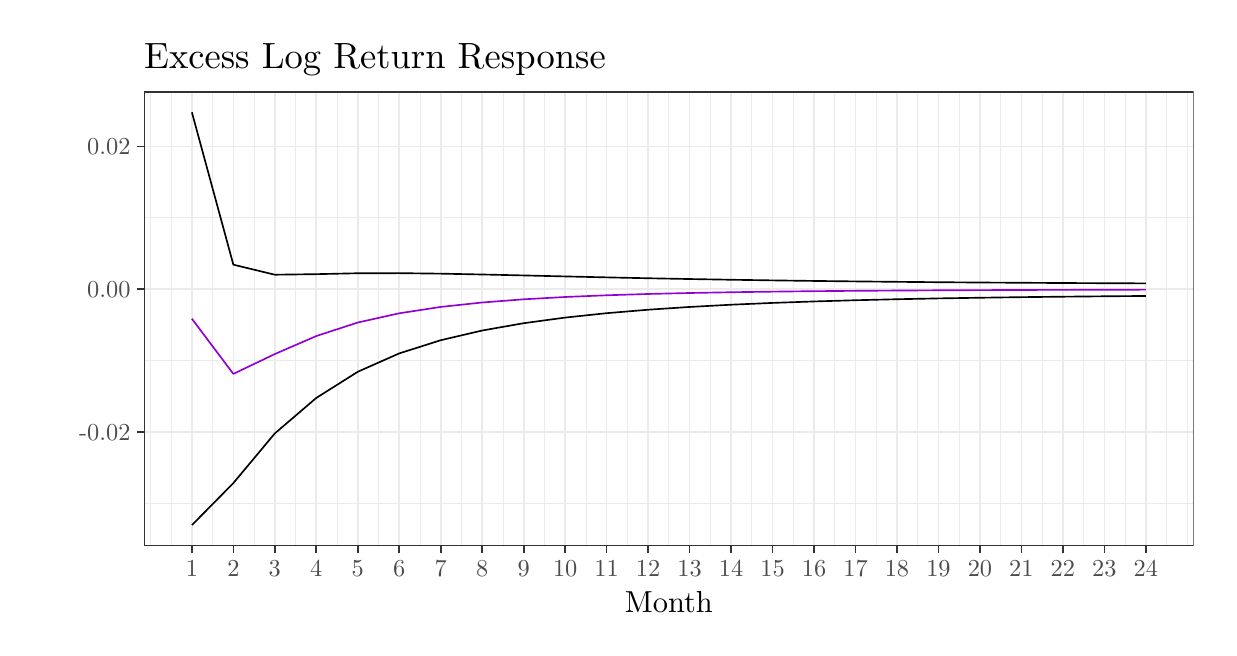
\begin{tikzpicture}[x=1pt,y=1pt]
\definecolor{fillColor}{RGB}{255,255,255}
\path[use as bounding box,fill=fillColor,fill opacity=0.00] (0,0) rectangle (426.79,216.81);
\begin{scope}
\path[clip] (  0.00,  0.00) rectangle (426.79,216.81);
\definecolor{drawColor}{RGB}{255,255,255}
\definecolor{fillColor}{RGB}{255,255,255}

\path[draw=drawColor,line width= 0.6pt,line join=round,line cap=round,fill=fillColor] (  0.00,  0.00) rectangle (426.79,216.81);
\end{scope}
\begin{scope}
\path[clip] ( 42.10, 29.59) rectangle (421.29,193.67);
\definecolor{fillColor}{RGB}{255,255,255}

\path[fill=fillColor] ( 42.10, 29.59) rectangle (421.29,193.67);
\definecolor{drawColor}{gray}{0.92}

\path[draw=drawColor,line width= 0.3pt,line join=round] ( 42.10, 44.92) --
	(421.29, 44.92);

\path[draw=drawColor,line width= 0.3pt,line join=round] ( 42.10, 96.53) --
	(421.29, 96.53);

\path[draw=drawColor,line width= 0.3pt,line join=round] ( 42.10,148.13) --
	(421.29,148.13);

\path[draw=drawColor,line width= 0.3pt,line join=round] ( 44.35, 29.59) --
	( 44.35,193.67);

\path[draw=drawColor,line width= 0.3pt,line join=round] ( 51.84, 29.59) --
	( 51.84,193.67);

\path[draw=drawColor,line width= 0.3pt,line join=round] ( 66.83, 29.59) --
	( 66.83,193.67);

\path[draw=drawColor,line width= 0.3pt,line join=round] ( 81.82, 29.59) --
	( 81.82,193.67);

\path[draw=drawColor,line width= 0.3pt,line join=round] ( 96.80, 29.59) --
	( 96.80,193.67);

\path[draw=drawColor,line width= 0.3pt,line join=round] (111.79, 29.59) --
	(111.79,193.67);

\path[draw=drawColor,line width= 0.3pt,line join=round] (126.78, 29.59) --
	(126.78,193.67);

\path[draw=drawColor,line width= 0.3pt,line join=round] (141.77, 29.59) --
	(141.77,193.67);

\path[draw=drawColor,line width= 0.3pt,line join=round] (156.76, 29.59) --
	(156.76,193.67);

\path[draw=drawColor,line width= 0.3pt,line join=round] (171.74, 29.59) --
	(171.74,193.67);

\path[draw=drawColor,line width= 0.3pt,line join=round] (186.73, 29.59) --
	(186.73,193.67);

\path[draw=drawColor,line width= 0.3pt,line join=round] (201.72, 29.59) --
	(201.72,193.67);

\path[draw=drawColor,line width= 0.3pt,line join=round] (216.71, 29.59) --
	(216.71,193.67);

\path[draw=drawColor,line width= 0.3pt,line join=round] (231.70, 29.59) --
	(231.70,193.67);

\path[draw=drawColor,line width= 0.3pt,line join=round] (246.68, 29.59) --
	(246.68,193.67);

\path[draw=drawColor,line width= 0.3pt,line join=round] (261.67, 29.59) --
	(261.67,193.67);

\path[draw=drawColor,line width= 0.3pt,line join=round] (276.66, 29.59) --
	(276.66,193.67);

\path[draw=drawColor,line width= 0.3pt,line join=round] (291.65, 29.59) --
	(291.65,193.67);

\path[draw=drawColor,line width= 0.3pt,line join=round] (306.63, 29.59) --
	(306.63,193.67);

\path[draw=drawColor,line width= 0.3pt,line join=round] (321.62, 29.59) --
	(321.62,193.67);

\path[draw=drawColor,line width= 0.3pt,line join=round] (336.61, 29.59) --
	(336.61,193.67);

\path[draw=drawColor,line width= 0.3pt,line join=round] (351.60, 29.59) --
	(351.60,193.67);

\path[draw=drawColor,line width= 0.3pt,line join=round] (366.59, 29.59) --
	(366.59,193.67);

\path[draw=drawColor,line width= 0.3pt,line join=round] (381.57, 29.59) --
	(381.57,193.67);

\path[draw=drawColor,line width= 0.3pt,line join=round] (396.56, 29.59) --
	(396.56,193.67);

\path[draw=drawColor,line width= 0.3pt,line join=round] (411.55, 29.59) --
	(411.55,193.67);

\path[draw=drawColor,line width= 0.3pt,line join=round] (419.04, 29.59) --
	(419.04,193.67);

\path[draw=drawColor,line width= 0.6pt,line join=round] ( 42.10, 70.73) --
	(421.29, 70.73);

\path[draw=drawColor,line width= 0.6pt,line join=round] ( 42.10,122.33) --
	(421.29,122.33);

\path[draw=drawColor,line width= 0.6pt,line join=round] ( 42.10,173.93) --
	(421.29,173.93);

\path[draw=drawColor,line width= 0.6pt,line join=round] ( 59.34, 29.59) --
	( 59.34,193.67);

\path[draw=drawColor,line width= 0.6pt,line join=round] ( 74.32, 29.59) --
	( 74.32,193.67);

\path[draw=drawColor,line width= 0.6pt,line join=round] ( 89.31, 29.59) --
	( 89.31,193.67);

\path[draw=drawColor,line width= 0.6pt,line join=round] (104.30, 29.59) --
	(104.30,193.67);

\path[draw=drawColor,line width= 0.6pt,line join=round] (119.29, 29.59) --
	(119.29,193.67);

\path[draw=drawColor,line width= 0.6pt,line join=round] (134.27, 29.59) --
	(134.27,193.67);

\path[draw=drawColor,line width= 0.6pt,line join=round] (149.26, 29.59) --
	(149.26,193.67);

\path[draw=drawColor,line width= 0.6pt,line join=round] (164.25, 29.59) --
	(164.25,193.67);

\path[draw=drawColor,line width= 0.6pt,line join=round] (179.24, 29.59) --
	(179.24,193.67);

\path[draw=drawColor,line width= 0.6pt,line join=round] (194.23, 29.59) --
	(194.23,193.67);

\path[draw=drawColor,line width= 0.6pt,line join=round] (209.21, 29.59) --
	(209.21,193.67);

\path[draw=drawColor,line width= 0.6pt,line join=round] (224.20, 29.59) --
	(224.20,193.67);

\path[draw=drawColor,line width= 0.6pt,line join=round] (239.19, 29.59) --
	(239.19,193.67);

\path[draw=drawColor,line width= 0.6pt,line join=round] (254.18, 29.59) --
	(254.18,193.67);

\path[draw=drawColor,line width= 0.6pt,line join=round] (269.16, 29.59) --
	(269.16,193.67);

\path[draw=drawColor,line width= 0.6pt,line join=round] (284.15, 29.59) --
	(284.15,193.67);

\path[draw=drawColor,line width= 0.6pt,line join=round] (299.14, 29.59) --
	(299.14,193.67);

\path[draw=drawColor,line width= 0.6pt,line join=round] (314.13, 29.59) --
	(314.13,193.67);

\path[draw=drawColor,line width= 0.6pt,line join=round] (329.12, 29.59) --
	(329.12,193.67);

\path[draw=drawColor,line width= 0.6pt,line join=round] (344.10, 29.59) --
	(344.10,193.67);

\path[draw=drawColor,line width= 0.6pt,line join=round] (359.09, 29.59) --
	(359.09,193.67);

\path[draw=drawColor,line width= 0.6pt,line join=round] (374.08, 29.59) --
	(374.08,193.67);

\path[draw=drawColor,line width= 0.6pt,line join=round] (389.07, 29.59) --
	(389.07,193.67);

\path[draw=drawColor,line width= 0.6pt,line join=round] (404.06, 29.59) --
	(404.06,193.67);
\definecolor{drawColor}{RGB}{148,0,211}

\path[draw=drawColor,line width= 0.6pt,line join=round] ( 59.34,111.63) --
	( 74.32, 91.71) --
	( 89.31, 98.87) --
	(104.30,105.38) --
	(119.29,110.27) --
	(134.27,113.60) --
	(149.26,115.90) --
	(164.25,117.50) --
	(179.24,118.65) --
	(194.23,119.49) --
	(209.21,120.11) --
	(224.20,120.58) --
	(239.19,120.93) --
	(254.18,121.21) --
	(269.16,121.42) --
	(284.15,121.59) --
	(299.14,121.72) --
	(314.13,121.82) --
	(329.12,121.91) --
	(344.10,121.97) --
	(359.09,122.03) --
	(374.08,122.07) --
	(389.07,122.11) --
	(404.06,122.14);
\definecolor{drawColor}{RGB}{0,0,0}

\path[draw=drawColor,line width= 0.6pt,line join=round] ( 59.34, 37.05) --
	( 74.32, 52.24) --
	( 89.31, 70.20) --
	(104.30, 83.02) --
	(119.29, 92.47) --
	(134.27, 99.11) --
	(149.26,103.87) --
	(164.25,107.38) --
	(179.24,110.02) --
	(194.23,112.05) --
	(209.21,113.64) --
	(224.20,114.89) --
	(239.19,115.89) --
	(254.18,116.70) --
	(269.16,117.35) --
	(284.15,117.88) --
	(299.14,118.32) --
	(314.13,118.68) --
	(329.12,118.98) --
	(344.10,119.22) --
	(359.09,119.43) --
	(374.08,119.60) --
	(389.07,119.74) --
	(404.06,119.86);

\path[draw=drawColor,line width= 0.6pt,line join=round] ( 59.34,186.22) --
	( 74.32,131.17) --
	( 89.31,127.54) --
	(104.30,127.74) --
	(119.29,128.07) --
	(134.27,128.10) --
	(149.26,127.92) --
	(164.25,127.62) --
	(179.24,127.28) --
	(194.23,126.92) --
	(209.21,126.58) --
	(224.20,126.26) --
	(239.19,125.98) --
	(254.18,125.72) --
	(269.16,125.49) --
	(284.15,125.29) --
	(299.14,125.12) --
	(314.13,124.97) --
	(329.12,124.83) --
	(344.10,124.72) --
	(359.09,124.63) --
	(374.08,124.54) --
	(389.07,124.47) --
	(404.06,124.41);
\definecolor{drawColor}{gray}{0.20}

\path[draw=drawColor,line width= 0.6pt,line join=round,line cap=round] ( 42.10, 29.59) rectangle (421.29,193.67);
\end{scope}
\begin{scope}
\path[clip] (  0.00,  0.00) rectangle (426.79,216.81);
\definecolor{drawColor}{gray}{0.30}

\node[text=drawColor,anchor=base east,inner sep=0pt, outer sep=0pt, scale=  0.88] at ( 37.15, 67.69) {-0.02};

\node[text=drawColor,anchor=base east,inner sep=0pt, outer sep=0pt, scale=  0.88] at ( 37.15,119.30) {0.00};

\node[text=drawColor,anchor=base east,inner sep=0pt, outer sep=0pt, scale=  0.88] at ( 37.15,170.90) {0.02};
\end{scope}
\begin{scope}
\path[clip] (  0.00,  0.00) rectangle (426.79,216.81);
\definecolor{drawColor}{gray}{0.20}

\path[draw=drawColor,line width= 0.6pt,line join=round] ( 39.35, 70.73) --
	( 42.10, 70.73);

\path[draw=drawColor,line width= 0.6pt,line join=round] ( 39.35,122.33) --
	( 42.10,122.33);

\path[draw=drawColor,line width= 0.6pt,line join=round] ( 39.35,173.93) --
	( 42.10,173.93);
\end{scope}
\begin{scope}
\path[clip] (  0.00,  0.00) rectangle (426.79,216.81);
\definecolor{drawColor}{gray}{0.20}

\path[draw=drawColor,line width= 0.6pt,line join=round] ( 59.34, 26.84) --
	( 59.34, 29.59);

\path[draw=drawColor,line width= 0.6pt,line join=round] ( 74.32, 26.84) --
	( 74.32, 29.59);

\path[draw=drawColor,line width= 0.6pt,line join=round] ( 89.31, 26.84) --
	( 89.31, 29.59);

\path[draw=drawColor,line width= 0.6pt,line join=round] (104.30, 26.84) --
	(104.30, 29.59);

\path[draw=drawColor,line width= 0.6pt,line join=round] (119.29, 26.84) --
	(119.29, 29.59);

\path[draw=drawColor,line width= 0.6pt,line join=round] (134.27, 26.84) --
	(134.27, 29.59);

\path[draw=drawColor,line width= 0.6pt,line join=round] (149.26, 26.84) --
	(149.26, 29.59);

\path[draw=drawColor,line width= 0.6pt,line join=round] (164.25, 26.84) --
	(164.25, 29.59);

\path[draw=drawColor,line width= 0.6pt,line join=round] (179.24, 26.84) --
	(179.24, 29.59);

\path[draw=drawColor,line width= 0.6pt,line join=round] (194.23, 26.84) --
	(194.23, 29.59);

\path[draw=drawColor,line width= 0.6pt,line join=round] (209.21, 26.84) --
	(209.21, 29.59);

\path[draw=drawColor,line width= 0.6pt,line join=round] (224.20, 26.84) --
	(224.20, 29.59);

\path[draw=drawColor,line width= 0.6pt,line join=round] (239.19, 26.84) --
	(239.19, 29.59);

\path[draw=drawColor,line width= 0.6pt,line join=round] (254.18, 26.84) --
	(254.18, 29.59);

\path[draw=drawColor,line width= 0.6pt,line join=round] (269.16, 26.84) --
	(269.16, 29.59);

\path[draw=drawColor,line width= 0.6pt,line join=round] (284.15, 26.84) --
	(284.15, 29.59);

\path[draw=drawColor,line width= 0.6pt,line join=round] (299.14, 26.84) --
	(299.14, 29.59);

\path[draw=drawColor,line width= 0.6pt,line join=round] (314.13, 26.84) --
	(314.13, 29.59);

\path[draw=drawColor,line width= 0.6pt,line join=round] (329.12, 26.84) --
	(329.12, 29.59);

\path[draw=drawColor,line width= 0.6pt,line join=round] (344.10, 26.84) --
	(344.10, 29.59);

\path[draw=drawColor,line width= 0.6pt,line join=round] (359.09, 26.84) --
	(359.09, 29.59);

\path[draw=drawColor,line width= 0.6pt,line join=round] (374.08, 26.84) --
	(374.08, 29.59);

\path[draw=drawColor,line width= 0.6pt,line join=round] (389.07, 26.84) --
	(389.07, 29.59);

\path[draw=drawColor,line width= 0.6pt,line join=round] (404.06, 26.84) --
	(404.06, 29.59);
\end{scope}
\begin{scope}
\path[clip] (  0.00,  0.00) rectangle (426.79,216.81);
\definecolor{drawColor}{gray}{0.30}

\node[text=drawColor,anchor=base,inner sep=0pt, outer sep=0pt, scale=  0.88] at ( 59.34, 18.58) {1};

\node[text=drawColor,anchor=base,inner sep=0pt, outer sep=0pt, scale=  0.88] at ( 74.32, 18.58) {2};

\node[text=drawColor,anchor=base,inner sep=0pt, outer sep=0pt, scale=  0.88] at ( 89.31, 18.58) {3};

\node[text=drawColor,anchor=base,inner sep=0pt, outer sep=0pt, scale=  0.88] at (104.30, 18.58) {4};

\node[text=drawColor,anchor=base,inner sep=0pt, outer sep=0pt, scale=  0.88] at (119.29, 18.58) {5};

\node[text=drawColor,anchor=base,inner sep=0pt, outer sep=0pt, scale=  0.88] at (134.27, 18.58) {6};

\node[text=drawColor,anchor=base,inner sep=0pt, outer sep=0pt, scale=  0.88] at (149.26, 18.58) {7};

\node[text=drawColor,anchor=base,inner sep=0pt, outer sep=0pt, scale=  0.88] at (164.25, 18.58) {8};

\node[text=drawColor,anchor=base,inner sep=0pt, outer sep=0pt, scale=  0.88] at (179.24, 18.58) {9};

\node[text=drawColor,anchor=base,inner sep=0pt, outer sep=0pt, scale=  0.88] at (194.23, 18.58) {10};

\node[text=drawColor,anchor=base,inner sep=0pt, outer sep=0pt, scale=  0.88] at (209.21, 18.58) {11};

\node[text=drawColor,anchor=base,inner sep=0pt, outer sep=0pt, scale=  0.88] at (224.20, 18.58) {12};

\node[text=drawColor,anchor=base,inner sep=0pt, outer sep=0pt, scale=  0.88] at (239.19, 18.58) {13};

\node[text=drawColor,anchor=base,inner sep=0pt, outer sep=0pt, scale=  0.88] at (254.18, 18.58) {14};

\node[text=drawColor,anchor=base,inner sep=0pt, outer sep=0pt, scale=  0.88] at (269.16, 18.58) {15};

\node[text=drawColor,anchor=base,inner sep=0pt, outer sep=0pt, scale=  0.88] at (284.15, 18.58) {16};

\node[text=drawColor,anchor=base,inner sep=0pt, outer sep=0pt, scale=  0.88] at (299.14, 18.58) {17};

\node[text=drawColor,anchor=base,inner sep=0pt, outer sep=0pt, scale=  0.88] at (314.13, 18.58) {18};

\node[text=drawColor,anchor=base,inner sep=0pt, outer sep=0pt, scale=  0.88] at (329.12, 18.58) {19};

\node[text=drawColor,anchor=base,inner sep=0pt, outer sep=0pt, scale=  0.88] at (344.10, 18.58) {20};

\node[text=drawColor,anchor=base,inner sep=0pt, outer sep=0pt, scale=  0.88] at (359.09, 18.58) {21};

\node[text=drawColor,anchor=base,inner sep=0pt, outer sep=0pt, scale=  0.88] at (374.08, 18.58) {22};

\node[text=drawColor,anchor=base,inner sep=0pt, outer sep=0pt, scale=  0.88] at (389.07, 18.58) {23};

\node[text=drawColor,anchor=base,inner sep=0pt, outer sep=0pt, scale=  0.88] at (404.06, 18.58) {24};
\end{scope}
\begin{scope}
\path[clip] (  0.00,  0.00) rectangle (426.79,216.81);
\definecolor{drawColor}{RGB}{0,0,0}

\node[text=drawColor,anchor=base,inner sep=0pt, outer sep=0pt, scale=  1.10] at (231.70,  5.50) {Month};
\end{scope}
\begin{scope}
\path[clip] (  0.00,  0.00) rectangle (426.79,216.81);
\definecolor{drawColor}{RGB}{0,0,0}

\node[text=drawColor,anchor=base west,inner sep=0pt, outer sep=0pt, scale=  1.32] at ( 42.10,202.22) {Excess Log Return Response};
\end{scope}
\end{tikzpicture}
